% myelin water imaging
\begin{comment}
\begin{frame}{%
	Background
	\footnote{%
		figure borrowed from
		\href{%
			https://www.mayoclinic.org/diseases-conditions/multiple-sclerosis/symptoms-causes/syc-20350269%
		}{%
			www.mayoclinic.org
		}% 
	}%
}%
	\begin{minipage}{0.54\textwidth}
		\uncover<2-3>{%
			Myelin water fraction (MWF): 
  		\begin{itemize}
  			\item<2->{%
  				MR signal fraction \\
					arising from water trapped \\
					within myelin bilayers \\
  				relative to total signal \\
					\hfill \citec{mackay:94:ivv}
  			}%
  			\item<3->{%
  				Correlates well \\
					with intact myelin content \\
					\hfill \citec{webb:03:imt}
  			}%
  		\end{itemize}
		}%
	\end{minipage}
	\begin{minipage}{0.4\textwidth}
		\uncover<1-3>{%
			\begin{figure}
				\centering
				\includegraphics[width=\textwidth]{c,mwf/myelin}
			\end{figure}
		}%
	\end{minipage}
\end{frame}
\end{comment}

\begin{frame}{Previous MW imaging acquisitions}
	\uncover<1>{%
  	Multi-echo spin-echo (\textbf{MESE}) \hfill \citec{mackay:94:ivv}
  	\begin{itemize}
  		\item{Considered a gold-standard}
  		\item{Speed-limited by long repetition times ($\sim$1-2s)}
  	\end{itemize}
  }%
  \uncover<2>{%
  	Combinations of fast steady-state scans using variable flip angles 
			(``\textbf{mcDESPOT}'') 
  		\hfill \citec{deoni:08:gmt}
  	\begin{itemize}
  		\item{Whole-brain, high-resolution MW imaging in $\sim$30m}
  		\item{%
  			Disagree with MESE MWF estimates \hfill \citec{zhang:15:com}
  			likely due to insufficient precision \hfill \citec{lankford:13:oti}
  		}%
  	\end{itemize}
	}%
	\uncover<3->{%
		\textbf{Goal}: fast, accurate MW content quantification in WM
	}%
\end{frame}

\begin{frame}{A voxel-scale MW content model}
	\begin{figure}
		\begin{tikzpicture}
			\uncover<1->{%
				\node[above] at (2,4) {simple two-compartment model};
				\draw[thick,fill=gray!10] (0,0) -- (2,0) -- (1,4) -- (0,4) -- (0,0);
				\draw[thick,fill=gray!30] (2,0) -- (4,0) -- (4,4) -- (1,4);
				\node[below] at (1,0) {``fast''};
				\node[below] at (3,0) {``slow''};
			}%
			\only<2-3>{%
				\node[below right] at (0,0.7) {$\tf{1},\tf{2}$};
				\node[below left] at (4,0.7) {$\ts{1},\ts{2}$};
  			\alt<2>{%
  				\node at (2.7,2) {$\paren{1-\ff}\mzero$};
  				\node at (0.7,2) {$\ff \mzero$};
  			}{%
  				\node at (2.7,2) {$\paren{1-\hlg{\ff}}\mzero$};
  				\node at (0.7,2) {$\hlg{\ff} \mzero$};
  			}%
			}%
		\end{tikzpicture}
	\end{figure}
	\uncover<3->{%
		Take fast-relaxing fraction $\hlg{\ff}$ as a simple measure of MW content
	}%
\end{frame}

\begin{frame}{Multi-compartmental MR signal models}
	\uncover<1-3>{%
		Two-compartment SPGR model \hfill \citec{spencer:00:mos}
	}%
	\begin{itemize}
		\item<1>{included first-order physical exchange}
		\item<1,4>{neglected relaxation, precession, exchange during excitation}
		\item<2,4>{%
			absorbing off-resonance effects into $\mzero$ 
			\emph{implies} neglecting exchange between excitation and readout
		}%
	\end{itemize}
	\uncover<3->{%
		Two-compartment DESS model \hfill \citec{nataraj:17:mwf}
	}%
	\begin{itemize}
		\item<3-4>{%
			additional approximations required 
			unless we assume time-independent diff 
			in compartmental off-resonance freq
		}%
		\item<4>{%
			including exchange, closed-form solutions still elusive
		}%
	\end{itemize}
	\uncover<5>{%
		\textbf{For simplicity, we use short echo times and neglect exchange.}
	}%
\end{frame}

\begin{frame}{Bayesian Acquisition Design}
	\begin{align}
    \breve{\bmP} &\in 
    	\set{%
        \argmin{\bmP \in \setP}
        \expcost\paren{\bmP}
    	}, \where \nonumber \\
		\expcost\paren{\bmP} &:=
    	\expect{\bmx,\bmnu}{\trace{\bmW \bmF^{-1}\paren{\bmx; \bmnu, \bmP} \bmW\tpose}}
  \end{align}
  \vspace{-0.5cm}
  \begin{itemize}
  	\item<2>{%
			\makebox[1.5cm][l]{$\bmx$} 
			$\brac{\hlg{\ff}, \tf{1}, \tf{2}, \ts{1}, \ts{2}, \mzero}\tpose$
		}%
		\item<2>{%
			\makebox[1.5cm][l]{$\bmnu$}
			transmit field spatial variation $\stx$
		}%
		\item<2>{%
			\makebox[1.5cm][l]{$\bmP$}
			SPGR/DESS nominal flip angles, repetition times
		}%
		\item<3>{%
			\makebox[1.5cm][l]{$\bmW$}
			$\diag{\brac{\inv{\expect{\bmx,\bmnu}{\hlg{\ff}}}, \zeros{5}\tpose}\tpose}$
		}%
		\item<4>{%
			\makebox[1.5cm][l]{$\expect{\bmx,\bmnu}{\cdot}$}
			approximated via empirical averages \\
			\makebox[1.5cm][l]{}
			of samples drawn from separable prior
		}%
		\item<5>{%
			\makebox[1.5cm][l]{$\setP$}
			nom flip angle, total scan time constraints
		}%
  \end{itemize}
\end{frame}

\begin{frame}{Optimized SPGR/DESS Acquisition}
	\begin{table}[!tb]
    \centering
    \begin{tabular}{r | c | c}
      \hline
      \hline
      & Optimized flip angles (deg) & Optimized rep. times (ms) \\
      \hline
    	SPGR & -- 										& -- \\
    	DESS & $33.0,18.3,15.1$ 			& $17.5,30.2,60.3$ \\
      \hline
      \hline
    \end{tabular}
    \caption{Optimized Scan Parameters, $\breve{\bmP}$}
		\label{tab:mwf,acq}
	\end{table}
	\vspace{-0.5cm}
	\begin{itemize}
		\item{%
			Predicted $\hlg{\ff}$ relative standard deviation in WM
			\begin{itemize} 
				\item{%
					Optimized SPGR/DESS:
					$\sqrt{\expcost\paren{\breve{\bmP}}} = 0.425$
				}%
				\item{%
					mcDESPOT: 
					at least $1$ \hfill \citec{lankford:13:oti}
				}%
			\end{itemize}
		}%
	\end{itemize}
\end{frame}

\begin{frame}{Simulation Studies}
	\uncover<1-3>{%
		Applied PERK for $\hlg{\ff}$ estimation from optimized DESS acquisition
	}%
	\uncover<2>{%
		\begin{itemize}
			\item{%
				PERK trained using $N\gets10^6$ samples 
				from prior dist $\dist{\bmx,\bmnu}$
			}%
			\item{%
				To enable precise estimation,
				$\dist{\bmx,\bmnu}$ chosen similar
				to Bayesian scan design sampling dist,
				but with finite support
			}%
		\end{itemize}
	}%
	\uncover<3->{%
		Compared DESS PERK $\hlg{\ff}$ estimates to:
	}%
	\begin{itemize}
		\item<3->{%
			DESS ML $\hlg{\ff}$ estimates \\
			(via VPM and unrealistically narrow grid search around truth)
		}%
		\item<4->{%
			MESE nonnegative least-squares (NNLS) MWF $\hlm{\mwf}$ estimates
		}%
		\item<4->{%
			MESE regularized NNLS (RNNLS) $\hlm{\mwf}$ estimates
		}%
	\end{itemize}
\end{frame}

\begin{frame}{Two-Compartment Simulation without Model Mismatch}
	\uncover<1>{%
		Simulated data to arise from \textbf{two} water compartments \\
		each with different nominal $\Tt$ values 
		but \textbf{same nominal $\To$ value}
		\begin{itemize}
			\item{%
				DESS $\hlg{\ff}$ estimates use known $\stx$
			}%
			\item{%
				MESE $\hlm{\mwf}$ estimates use known $\stx$, bulk $\To$
			}%
		\end{itemize}
	}%
	\uncover<2>{%
		Since no model mismatch, 
		$\hlg{\ff}$ and $\hlm{\mwf}$ estimates are comparable
	}%
\end{frame}

\begin{frame}{Two-Compartment Simulation Result}
	\vspace{-0.3cm}
	\begin{figure}
		\centering
		\begin{minipage}{\textwidth}
			\subfloat{%
				\includegraphics [width=\textwidth] {%
					c,mwf/2comp/mese-mw,dess-ff,sl-81,im.eps%
				}%
				\label{fig:mwf,2comp,im}
			}%
			\hspace{0cm}
			\subfloat{%
				\includegraphics [width=\textwidth,trim=0 0 0 25,clip] {%
					c,mwf/2comp/mese-mw,dess-ff,sl-81,err.eps%
				}%
				\label{fig:mwf,2comp,err}
			}%
		\end{minipage}
		\label{fig:mwf,2comp}
	\end{figure}
	\vspace{-0.5cm}
	\uncover<2->{%
		\makebox[2.2cm][r]{estimation time:}
		\makebox[3.3cm][c]{}
		\makebox[1.65cm][c]{$\sim$5h}
		\makebox[1.8cm][r]{$33.8$s train} \\
		\vspace{-0.1cm}
		\makebox[7.15cm][c]{}
		\makebox[1.9cm][r]{$1.0$s test} \\
	}%
	\uncover<3->{%
		\vspace{0.5cm}
		\makebox[2.2cm][r]{WM RMSE:}
		\makebox[1.65cm][c]{$0.0225$}
		\makebox[1.65cm][c]{$0.0260$}
		\makebox[1.65cm][c]{$0.0433$}
		\makebox[1.65cm][c]{$0.0305$}
	}%
\end{frame}

\begin{frame}{Three-Compartment Simulation with Model Mismatch}
	\uncover<1>{%
		Next simulated data to arise from \textbf{three} water compartments \\
		each with different nominal $\Tt$ \textbf{and $\To$ values}
		\begin{itemize}
			\item{%
				DESS $\hlg{\ff}$ estimators now incur bias \\
				due to two-compartment model assumption
			}%
			\item{%
				MESE $\hlm{\mwf}$ estimators now incur bias \\
				due to bulk-$\To$ model assumption (significant for $\TR\sim1$s)
			}%
		\end{itemize}
	}%
	\uncover<2>{%
		Due to model mismatch, \\
		$\hlg{\ff}$ and $\hlm{\mwf}$ estimates \textbf{need not be comparable}.
	}%
\end{frame}

\begin{frame}{Three-Compartment Simulation Result}
	\vspace{-0.3cm}
	\begin{figure}
		\centering
		\begin{minipage}{\textwidth}
			\subfloat{%
				\includegraphics [width=\textwidth] {%
					c,mwf/3comp/mese-mw,dess-ff,sl-81,im.eps%
				}%
				\label{fig:mwf,3comp,im}
			}%
			\hspace{0cm}
			\subfloat{%
				\includegraphics [width=\textwidth,trim=0 0 0 25,clip] {%
					c,mwf/3comp/mese-mw,dess-ff,sl-81,err.eps%
				}%
				\label{fig:mwf,3comp,err}
			}%
		\end{minipage}
		\label{fig:mwf,3comp}
	\end{figure}
	\vspace{-0.5cm}
	\uncover<1->{%
		\makebox[2.2cm][r]{estimation time:}
		\makebox[3.3cm][c]{}
		\makebox[1.65cm][c]{$\sim$5h}
		\makebox[1.8cm][r]{$34.2$s train} \\
		\vspace{-0.1cm}
		\makebox[7.15cm][c]{}
		\makebox[1.9cm][r]{$1.1$s test} \\
	}%
	\uncover<2->{%
		\vspace{0.5cm}
		\makebox[2.2cm][r]{WM RMSE:}
		\makebox[1.65cm][c]{$0.0618$}
		\makebox[1.65cm][c]{$0.0406$}
		\makebox[1.65cm][c]{$0.0559$}
		\makebox[1.65cm][c]{$0.0254$}
	}%
\end{frame}

\begin{frame}{\Invivo Experiment}
	\uncover<1-3>{%
		In a single long study of a healthy volunteer:
	}%
	\begin{itemize}
		\item<1-3>{%
			Precision-optimized DESS acquisition
		}%
		\item<2-3>{%
			32-echo MESE acquisition
			\begin{itemize}
				\item{%
					Used shaped refocusing pulses \\
					to suppress out-of-slab signal
					due to imperfect refocusing
				}%	
				\item{%
					Used shorter $\TR\gets600$ms 
					to limit scan time \\
					(compensated for incomplete recovery 
					w/ separate bulk-$\To$ est)
				}%
				\item{%
					Repeated acquisition twice
					to increase SNR through averaging
				}%
			\end{itemize}
		}%
		\item<3>{%
			BS acquisition for separate $\stx$ estimation
		}%
		\item<3>{%
			Variable-flip SPGR acquisition for separate bulk $\To$ estimation
		}%
	\end{itemize}
	\uncover<4>{%
		Compared DESS PERK $\hlg{\ff}$ estimates to:
	}%
	\begin{itemize}
		\item<4>{%
			MESE NNLS $\hlm{\mwf}$ estimates
		}%
		\item<4>{%
			MESE RNNLS $\hlm{\mwf}$ estimates
		}%
	\end{itemize}
\end{frame}
	
\begin{frame}{\Invivo Results}
	\begin{figure}
		\centering
		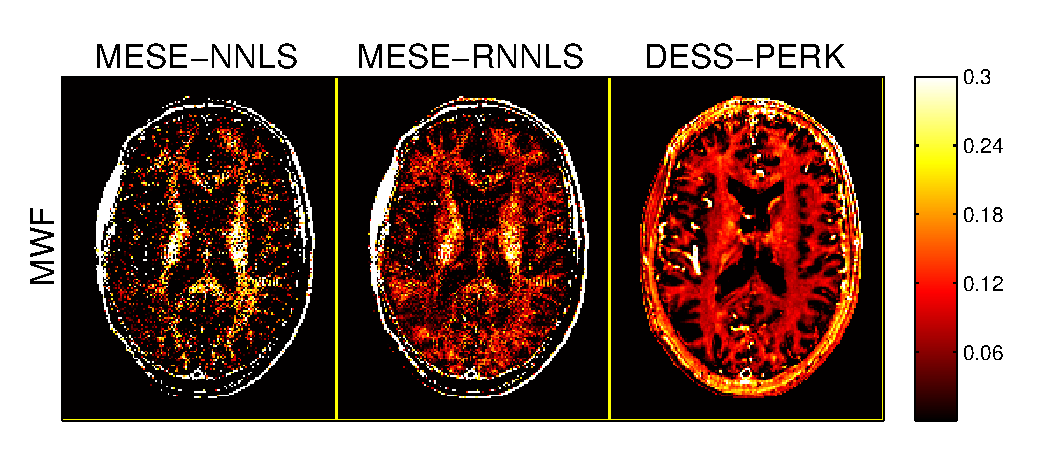
\includegraphics [width=\textwidth] {%
			c,mwf/brain/mese-mw,dess-ff,sl-5.eps%
		}%
		\label{fig:mwf,invivo}
	\end{figure}
	\vspace{-0.5cm}
	\uncover<2->{%
		\makebox[0.3cm][r]{scan} \\
		\vspace{-0.1cm}
		\makebox[0.4cm][r]{time:}
		\makebox[2.75cm][c]{$40$m$6$s}
		\makebox[2.75cm][c]{$40$m$6$s}
		\makebox[2.75cm][c]{$7$m$45$s}
	}%
\end{frame}	

\begin{frame}{Summary}
	\uncover<1-5>{%
  	\textbf{Contribution}
  	\begin{itemize}
  		\item<1->{Fast SS MRI acquisition for precise MW imaging}
			\begin{itemize}
				\item<2-3>{%
					Idealized simulations demonstrate
					that PERK and ML $\hlg{\ff}$ estimates are comparable
					but PERK is more than $500\times$ faster.
				}%
				\item<3>{%
					More realistic simulations demonstrate
					that both MESE $\hlg{\mwf}$ and DESS $\hlm{\ff}$ estimates
					are sensitive to model mismatch.
				}%
				\item<4->{%
					\Invivo experiments are the first to demonstrate \\
					lateral WM MW content estimates from a SS acquisition \\
					that are similar to conventional MESE MWF estimates.
				}%
			\end{itemize}
  	\end{itemize}
	}%
	\uncover<5->{%
		\textbf{Future Work}
		\begin{itemize}
			\item<5->{Investigate DESS $\hlg{\ff}$ accuracy in \exvivo studies}
			\item<5->{Correlate with other myelin biomarkers}
			\item<6->{Exploit off-resonance for MW imaging}
			\item<7->{Combine PERK with image reconstruction}
		\end{itemize}
	}%
\end{frame}
